\documentclass[aspectratio=169]{beamer} %[aspectratio=169]
\usetheme{Boadilla}
\usecolortheme{seahorse}

\usepackage{parskip}

% հայկական և լատինական տառատեսակի կարգավորում
\usepackage{fontspec}
% \usepackage{polyglossia}
% \setdefaultlanguage{armenian}
% \newfontfamily\armenianfont{GHEA Mariam}
\setmainfont{DejaVu Serif}
\setsansfont{DejaVu Sans}
\setmonofont{DejaVu Sans Mono}
% \setmainfont{/home/srohund/Documents/1991/Arti Regular.otf}

% մաթեմի տառատեսակ
\usepackage{unicode-math}
% Set the math font to Fira Math

% Գույների համար
\usepackage{xcolor}
\definecolor{seahorseblue}{RGB}{0, 102, 204}
\definecolor{seahorsered}{RGB}{204, 0, 0}
\definecolor{seahorsegreen}{RGB}{0, 153, 0}
\definecolor{seahorseyellow}{RGB}{255, 204, 0}

\definecolor{seahorseblue2}{RGB}{0, 105, 148}
\definecolor{seahorsegreen2}{RGB}{0, 128, 71}
\definecolor{seahorsered2}{RGB}{217, 0, 27}
\definecolor{seahorseorange2}{RGB}{255, 123, 0}
\definecolor{seahorsegray2}{RGB}{92, 92, 92}
\definecolor{seahorsepink2}{RGB}{214, 0, 96}
\definecolor{seahorseyellow2}{RGB}{255, 201, 0}

% հղումների համար
\usepackage{hyperref}
\hypersetup{
	colorlinks=true,
	linkcolor=seahorsered,
	urlcolor=seahorseblue,
	citecolor=seahorsegreen,
}

% պատկերներ
\usepackage{graphicx}
\graphicspath{ {./images/} } % \includegraphics


% հատուկ հրաման մեջտեղում գրելու համար
\newcommand{\tabitem}{%
  \usebeamertemplate{itemize item}\hspace*{\labelsep}}

% հիմնական տվյալներ
\title[մաթ․ անալիզ - դաս 2]{1991 ստորաբաժանման դիմորդների նախապատրաստական դասընթաց}
\subtitle{Մաթեմաթիկական անալիզի ներածություն, դաս 2}
\author[Առաքելյան Ա․]{
    \href{mailto:aram.arakeljan@gmail.com}{Առաքելյան Արամ}
}
\institute{\href{https://1991.mil.am/}{«1991» ակադեմիա}}

\date{2023թ դեկտեմբեր}
\begin{document}
    % գլխարկ
    \begin{frame}
        \titlepage
	% \maketitle
    \end{frame}
    % \begin{frame}
    %     \frametitle{Նախորդ դասին}
    %     \centering
    %     Շուտով․․․
    % \end{frame}
     %%%%%%%   բովանդականություն   %%%%%%%
    \begin{frame}
        \frametitle{Բովանդականություն}
        \begin{block}{}
            Իրական թվերի սահմանումը
            \begin{itemize}
                \item{Կառուցողական սահմանումներ}
                \item{Աքսիոմատիկ սահմանում}
            \end{itemize}
        \end{block}
        \begin{block}{}
            Իրական թվերի հատկությունները
            \begin{itemize}
                \item{Արամատ երկու, իռացիոնալ թվեր}
                \item{Ճշգրիտ վերին եզրի գոյությունը}
                \item{Ներդրված հատվածների լեմմ}
                \item{Իրական թվերի անհաշվելիությունը}
            \end{itemize}
        \end{block}
    \end{frame}
    \begin{frame}
        \frametitle{Իրական թվեր}
        \framesubtitle{Պատմական ակնարկ}
        \only<2->{
            \begin{block}{}
                Իրական թվերի առաջին նկարագրություններից է մեկը ներկայացված է Էվկլիդեսի «Սկզբունքներ» աշխատության մեջ, մոտ մ․թ․ա $3$-րդ դատրում։\\
                Իրական թվերին տրվում է երկրաչափական նկարագրություն՝ հատվածի երկարություն, պատկերի մակերես կամ մարմնի ծավալ։
            \end{block}
        }
        \only<3->{
            \begin{block}{}
                Միայն 1872թ տրվում է իրական թվերի մաթեմատիկական սահմանումը։ Իրական թվերը սահմանում են Կանտորը, Վայերշտրաս և Դեդեկինդը։
            \end{block}
        }
        \centering{
            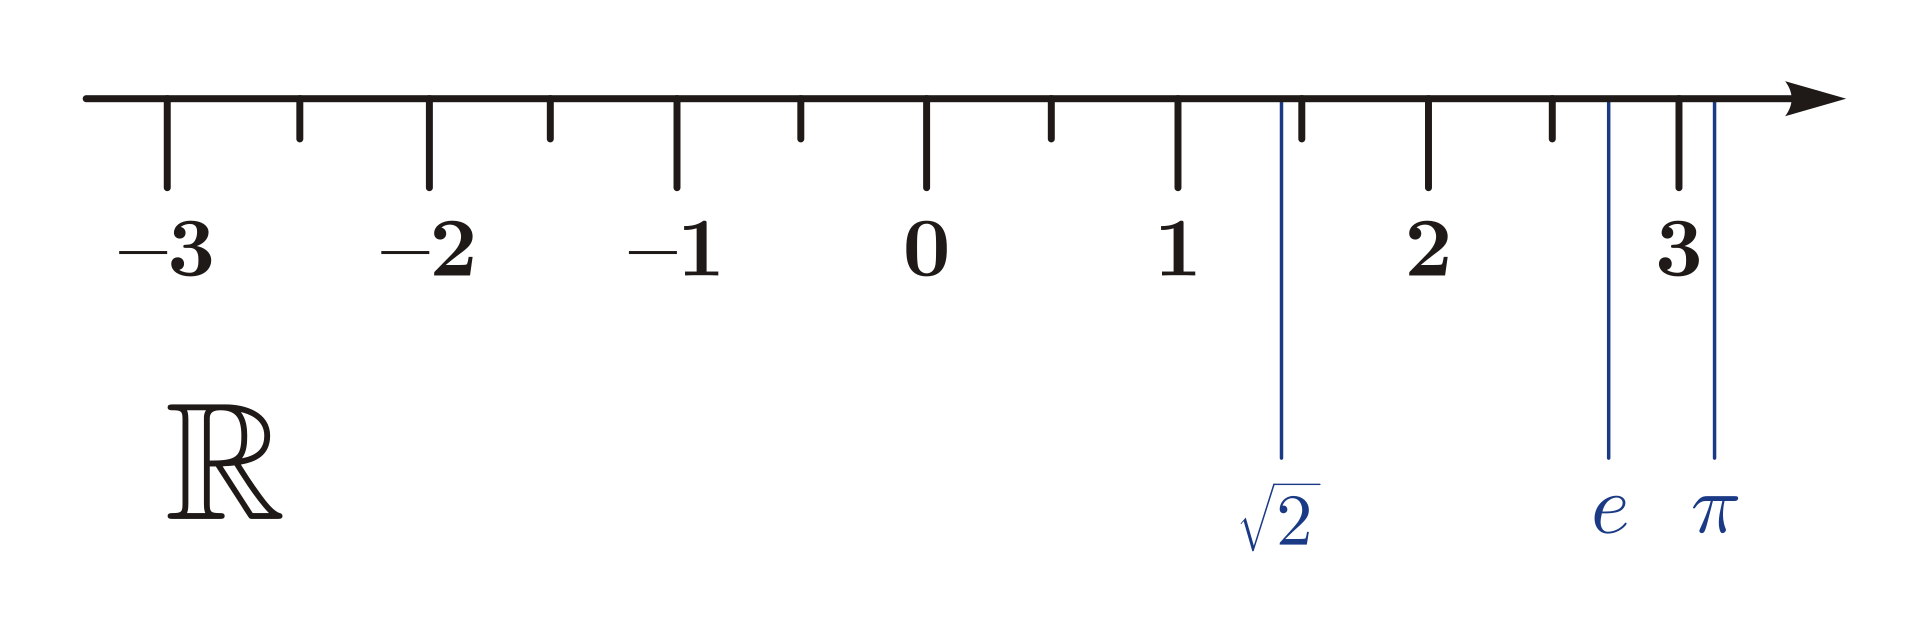
\includegraphics[width=0.4\textwidth]{real_number_line.png}
        }
        
    \end{frame}
    \begin{frame}
        \frametitle{Իրական թվեր}
        \framesubtitle{Սահմանումը}
        \only<2->{
            \begin{block}{Կառուցողական}
                \begin{itemize}
                    \item<2->{Կանտորի կառուցումը՝\\ հիմք են հանդիսանում ֆունդամետալ հաջորդականությունները}
                    \item<3->{Վայերշտրասի կառուցումը՝\\ հիմք են հանդիսանում անվերջ տասնորդական կոտորակները}
	                    \item<4->{Դեդեկինդը կառուցումը՝\\ հիմք են հանդիսանում ռացիոնալ թվերի բազմության հատույթները}
                \end{itemize}
            \end{block}
        }
        \only<5->{
            \begin{exampleblock}{Աքսիոմատիկ}
                Կարևոր չէ առարկաների էությունը, կարևոր է միայն գոյություն ունեցող հարաբերությունները նրանց միչև։
                \only<6->{
                    \begin{itemize}
                        \item<6->{հանրահաշվական կառուցվածքի աքսիոմներ}
                        \item<7->{կարգավորվածության աքսիոմներ}
                        \item<8->{անընդհատության աքսիոմներ}
                    \end{itemize}
                }
            \end{exampleblock}
        }
    \end{frame}
    \begin{frame}
        \frametitle{Իրական թվեր}
        \framesubtitle{Սահմանումը ըստ Կանտորի}
        \only<1-5>{Իրական թվերի նախատիպ է հանդիսանում Ֆունդամենտալ \alert<2-3>{ռացիոնալ հաջորդականությունը}\only<6->{։\\}}
        \only<3-5>{
            \only<3->{\[a: \mathbb{N} \rightarrow \alert<3>{\mathbb{Q}}\]}
            \only<4->{\[\mathbb{Q} = \left\{\frac{m}{n}: \; m \in \mathbb{Z}, n \in \mathbb{N}\right\}\]}
            \only<5->{
                \begin{center}
                    \renewcommand{\arraystretch}{1.5} % Adjust vertical spacing
                    % \setlength{\tabcolsep}{5pt} % Adjust horizontal spacing
                    \begin{matrix}
                        \frac{0}{1} & \frac{1}{1} & \frac{-1}{1} & \frac{2}{1} & \frac{-2}{1} & \frac{3}{1} & \frac{-3}{1} & \frac{4}{1} & \frac{-4}{1} & \dotsb \\
                        \frac{0}{2} & \frac{1}{2} & \frac{-1}{2} & \frac{2}{2} & \frac{-2}{2} & \frac{3}{2} & \frac{-3}{2} & \frac{4}{2} & \frac{-4}{2} & \dotsb \\
                        \frac{0}{3} & \frac{1}{3} & \frac{-1}{3} & \frac{2}{3} & \frac{-2}{3} & \frac{3}{3} & \frac{-3}{3} & \frac{4}{3} & \frac{-4}{3} & \dotsb \\
                        \frac{0}{4} & \frac{1}{4} & \frac{-1}{4} & \frac{2}{4} & \frac{-2}{4} & \frac{3}{4} & \frac{-3}{4} & \frac{4}{4} & \frac{-4}{4} & \dotsb \\
                        \frac{0}{5} & \frac{1}{5} & \frac{-1}{5} & \frac{2}{5} & \frac{-2}{5} & \frac{3}{5} & \frac{-3}{5} & \frac{4}{5} & \frac{-4}{5} & \dotsb \\
                        \vdots & \vdots & \vdots & \vdots & \vdots & \vdots & \vdots & \vdots & \vdots & \ddots \\
                    \end{matrix}
                \end{center}
            }
        }
        \only<5-9>{
            \begin{alertblock}{\only<9->{Առաջին տարբերակ}}
                \textcolor<-8>{seahorsegreen2}{$(a_n)$} և \textcolor<-8>{seahorseorange2}{$(b_n)$} ֆունդամենտալ հաջորդականությունները նույն թվի նախատիպն են, եթե․ \textcolor<-8>{seahorseblue2}{$(c_n)$} հաջորդականությունը ևս ֆունդամենտալ է, որտեղ.
                \[
                    c_n = 
                    \begin{cases}
                        a_n &\text{ երբ } n = 2k,\\
                        b_n &\text{ երբ } n = 2k - 1:\\
                    \end{cases}
                \]
            \end{alertblock}
            \only<-8>{\begin{center}
                \only<6>{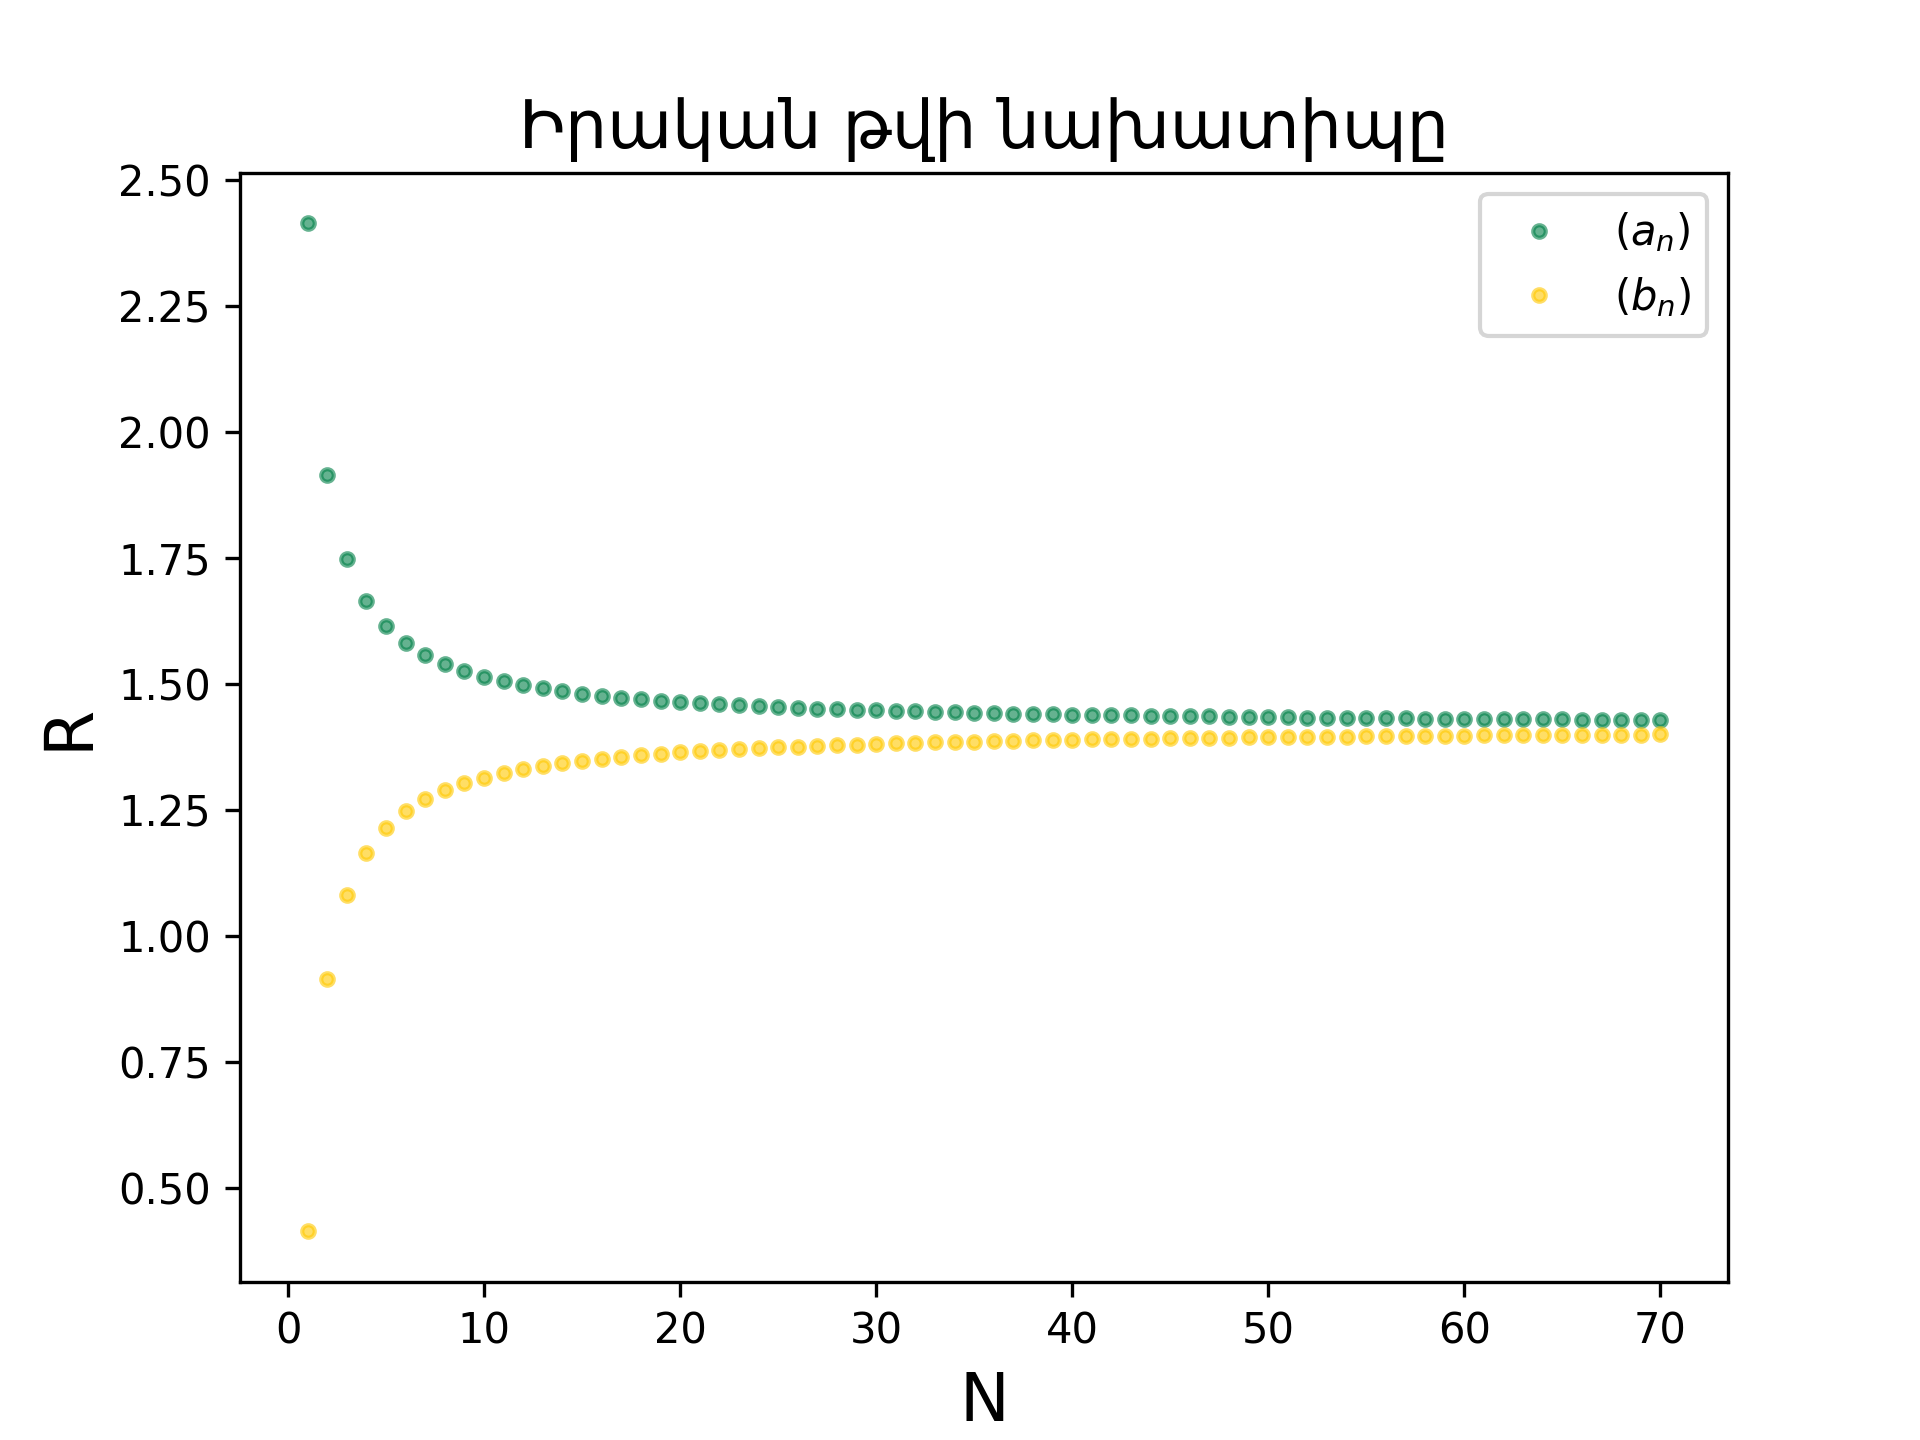
\includegraphics[width=0.35\textwidth]{equivalent_sequences_0.png}}
                \only<7>{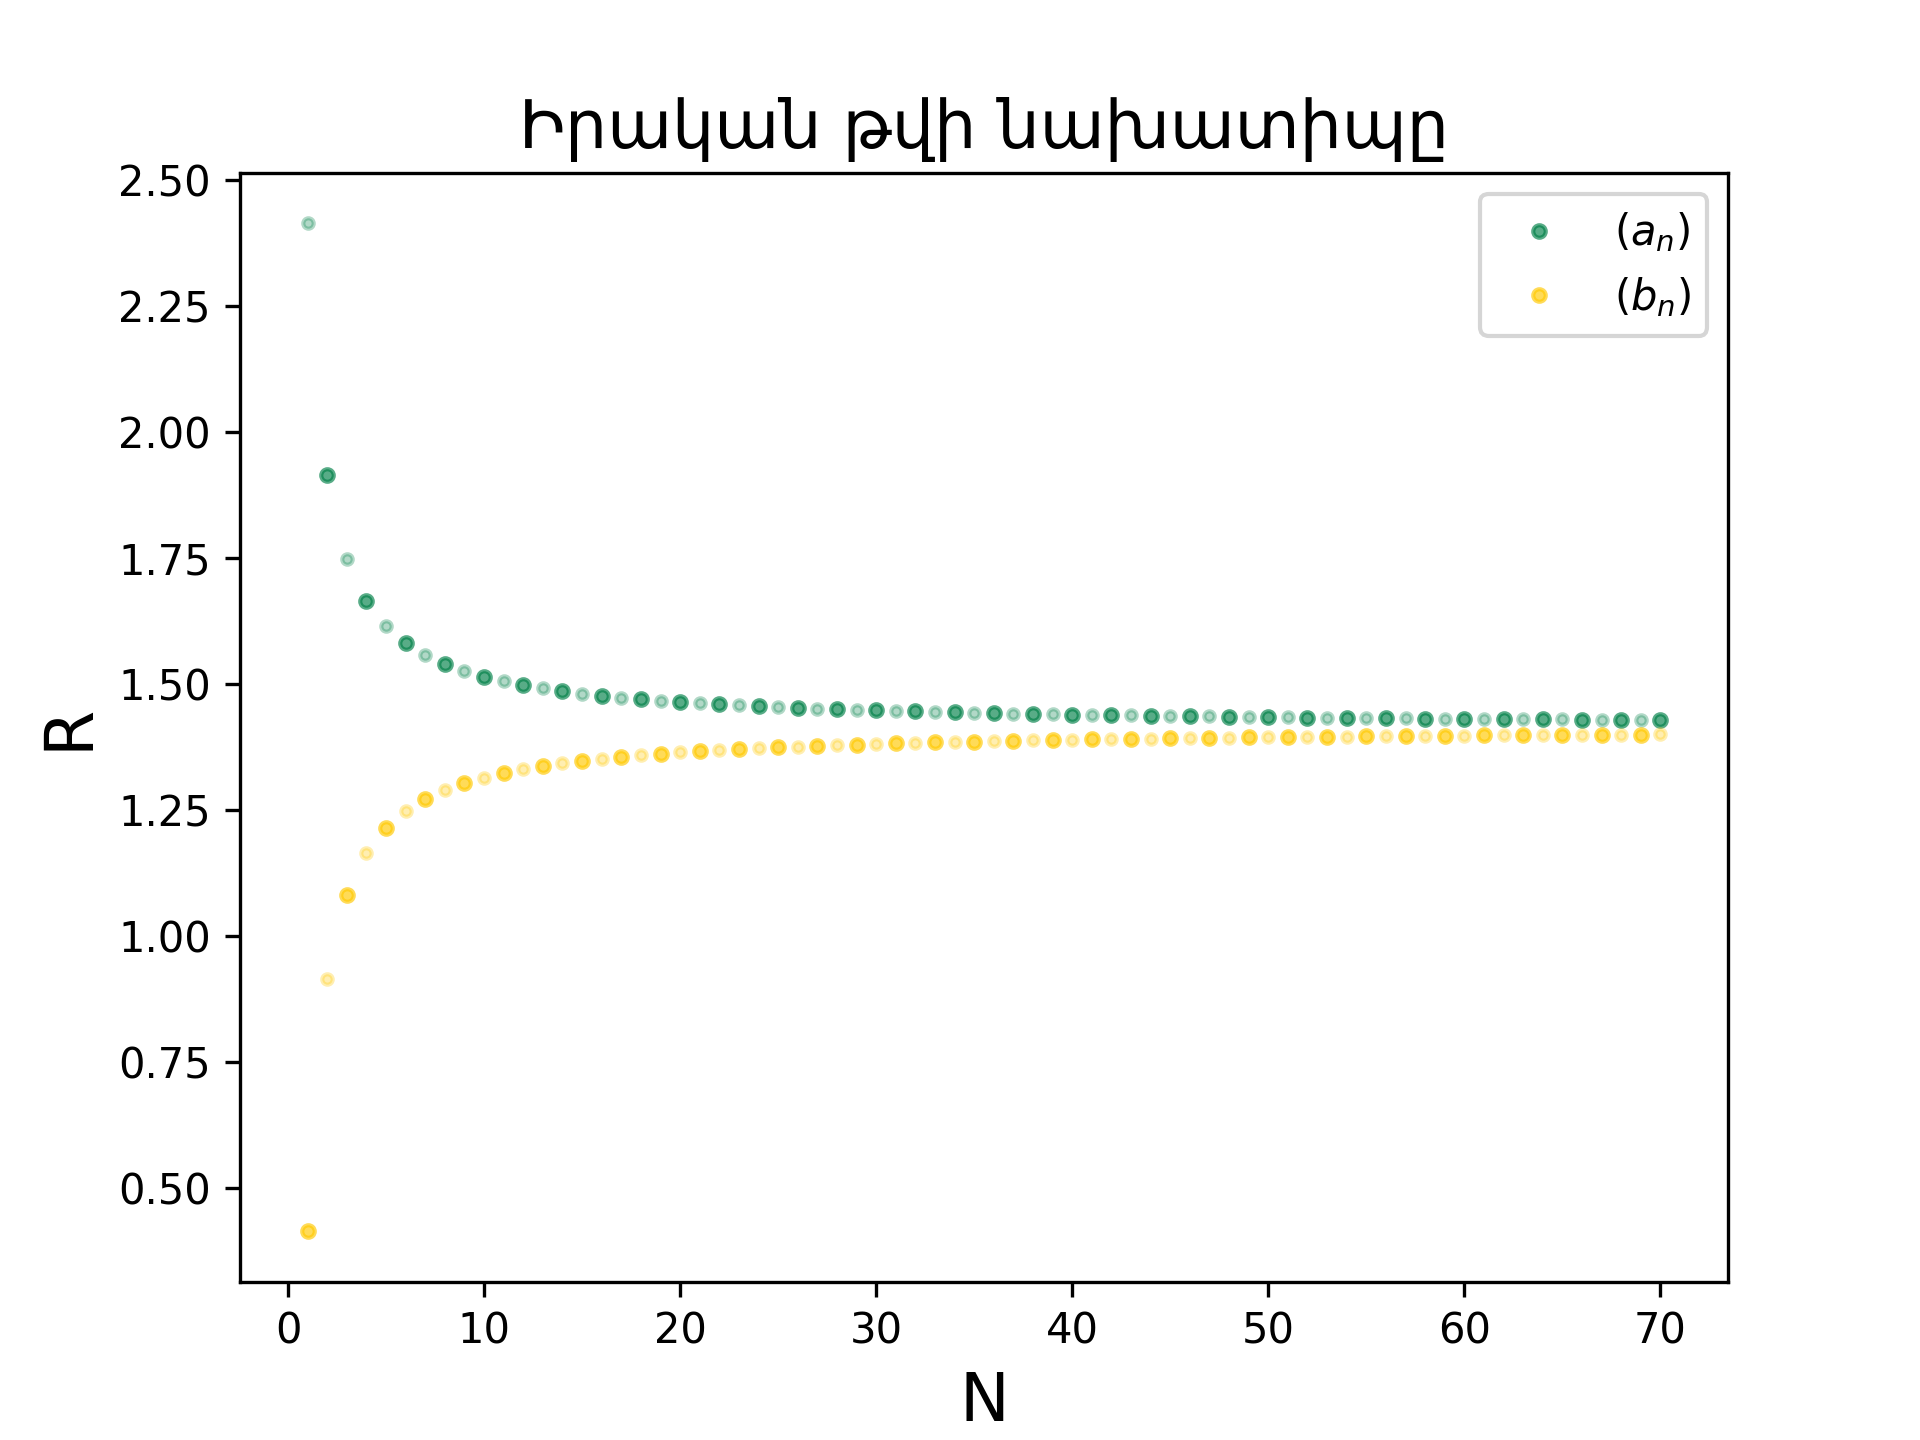
\includegraphics[width=0.35\textwidth]{equivalent_sequences_1.png}}
                \only<8>{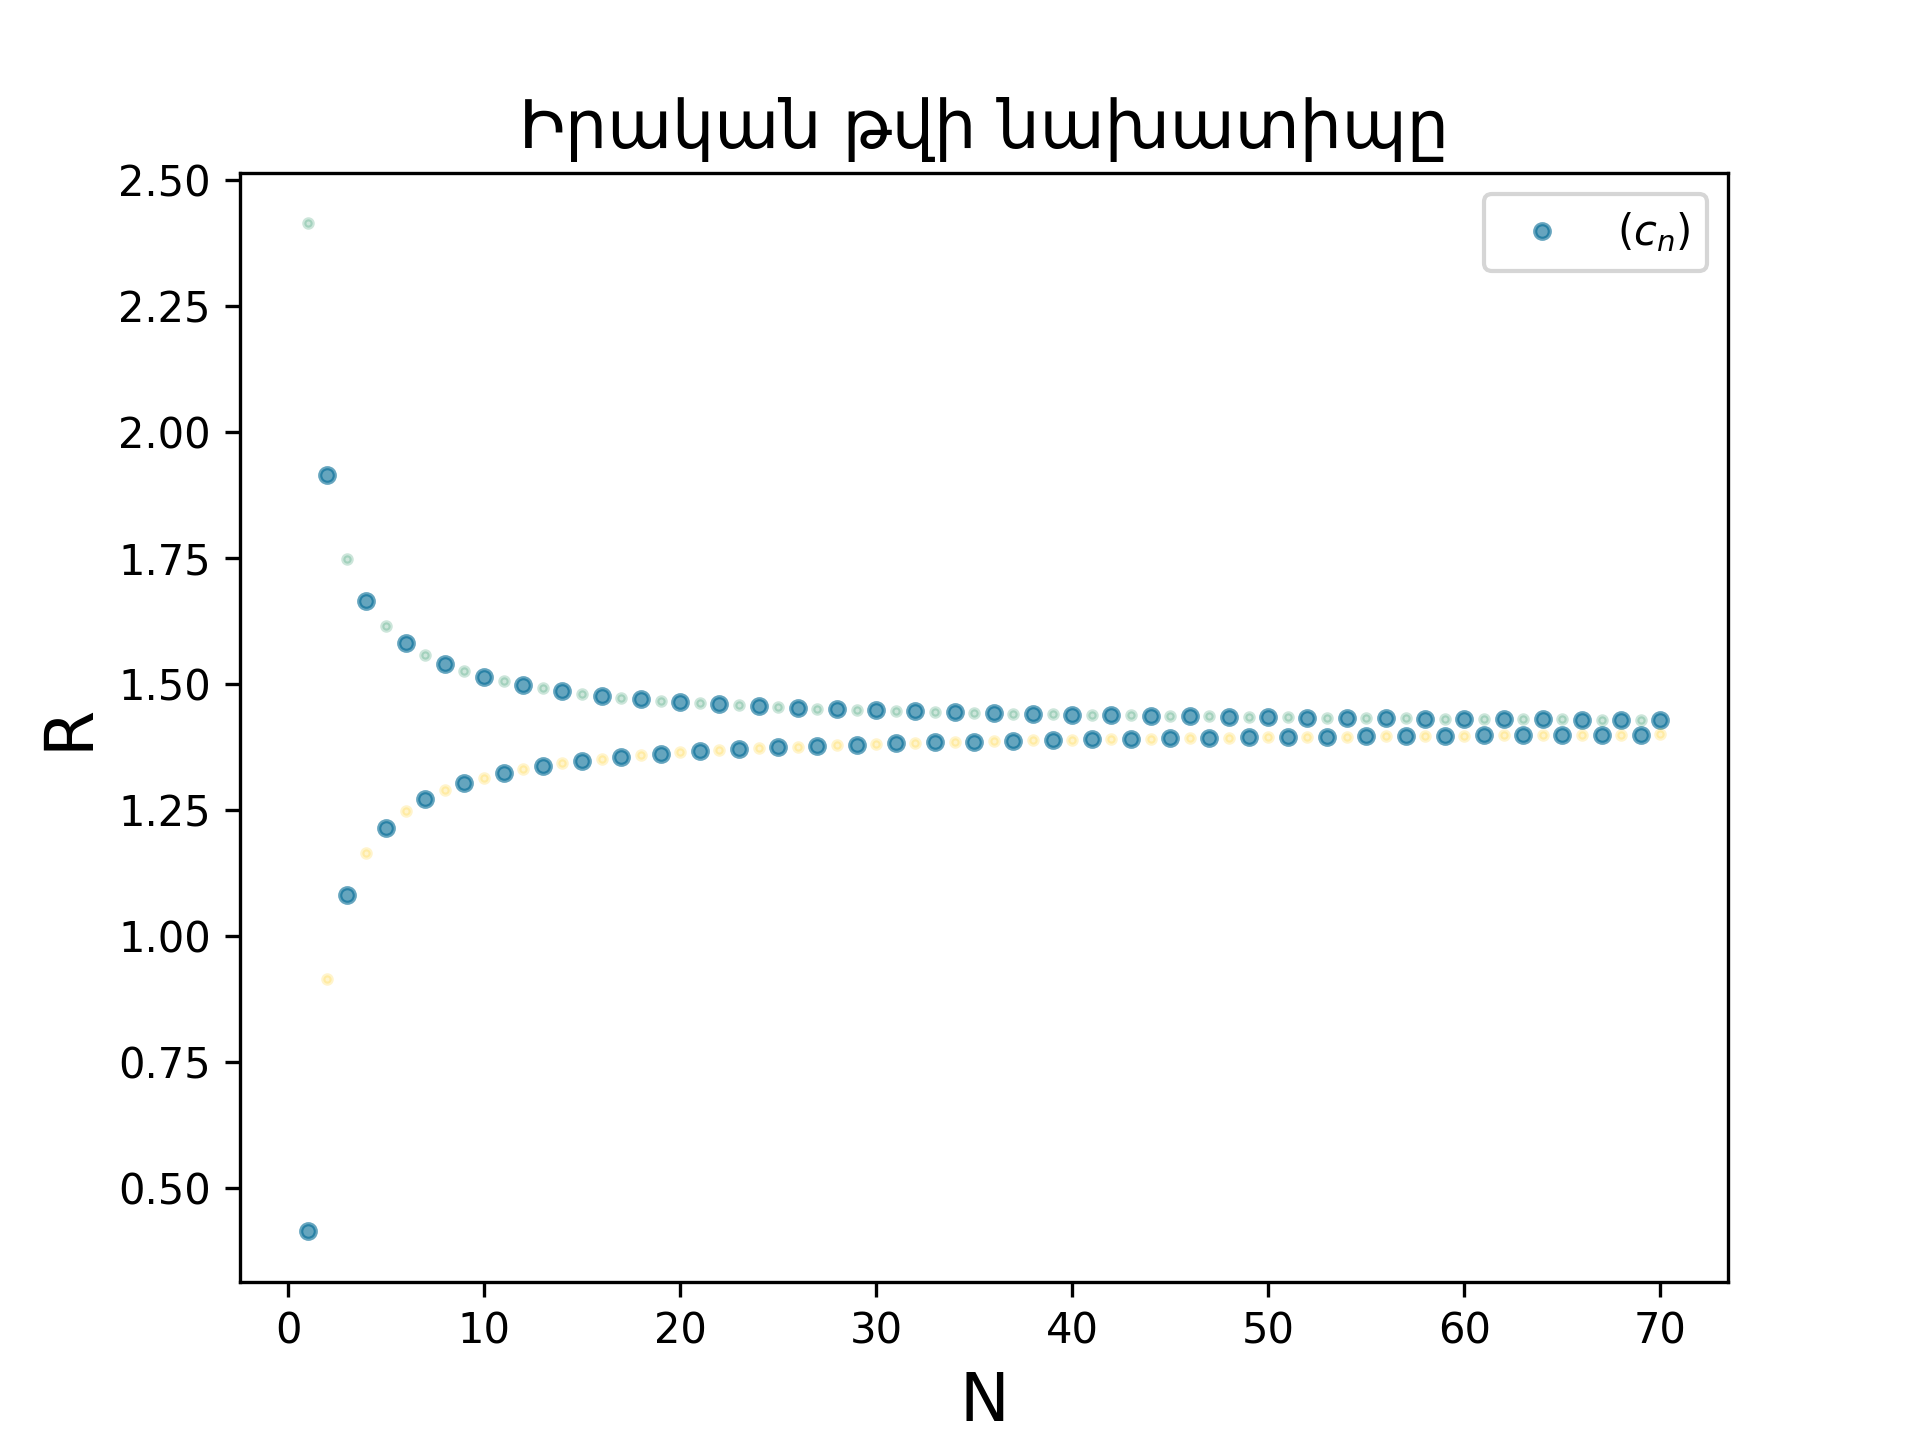
\includegraphics[width=0.35\textwidth]{equivalent_sequences_2.png}}
            \end{center}}
        }
        \only<9->{
            \begin{alertblock}{\only<-9>{Երկրորդ տարբերակ}}
                Երկու ֆունդամենտալ հաջորդականություն նույն իրական թվի նախատիպն են, եթե դրանց տարբերություն բացարձակ արժեքը \alert<10>{ինչքան ասես փոքր է} \alert<11>{ինչ֊որ պահից սկսած}.
                \[\alert<10>{\forall \varepsilon > 0} \; \alert<11>{\exists N_\varepsilon \in \mathbb{N} \; \forall n > N_\varepsilon}: \; |a_n - b_n| \alert<10>{< \varepsilon}:\]
            \end{alertblock}
        }
        \only<12-14>{
                \begin{exampleblock}{Օրինակ}
                    \only<12->{$a_n=\frac{1}{n}$ և $b_n=\frac{2}{n}$ հաջորդականությունները նույն թվի նախատիպն են։}
                    \only<13->{\[|a_n - b_n| = \frac{1}{n} < \varepsilon \text{ երբ } n > \frac{1}{\varepsilon}\]}
                    \only<14->{Այսինքն՝ \[\forall \varepsilon > 0\; \forall n > N_\varepsilon = \left[\frac{1}{\varepsilon}\right] + 1\; |a_n - b_n| < \varepsilon\]}
                \end{exampleblock}
        }
        \only<15->{
            \begin{block}{}
                Ֆունդամետալ հաջորդականությունների հանրահաշվական գրոծողությունները հանդիսանում են գործողություններ իրական թվերի համար։
            \end{block}
        }
    \end{frame}
    \begin{frame}
        \frametitle{Իրական թվեր}
        \framesubtitle{Սահմանումը ըստ Վայերշտրասի}
        \only<1>{\[3.14159265358979323846264338327950288419716939937510582097494...\]}
        \only<2-6>{
            Իրական թիվը հանդիսանում է անվերջ տասնորդական արտահայտություն հետևյալ տեսքի․
            \[\pm x_0.x_1x_2x_3x_4x_5x_6x_7x_8x_9x_{10}x_{11}x_{12}...,\]
            որտեղ $x_0 \in \mathbb{N}$, իսկ $x_1, x_2, ... \in \{0, 1, ... 9\}$։
        }
        \only<3-4>{
            \begin{exampleblock}{}
                Դիցուք $\alpha = \alert<4>{+}x_0.x_1x_2x_3...$: Ըստ Կանտորի կառուցման $\alpha$ թվի նախատիպ է հանդիսանում $(a_n)$ ֆունդամենտալ հաջորդականությունը, որտեղ․
                \[a_n = x_0.x_1...x_n = \frac{[\alpha 10^n]}{10^n} = x_0 \alert<4>{+} \frac{1}{10}x_1 \alert<4>{+} \frac{1}{10^2}x_2 \alert<4>{+} ... \alert<4>{+}\frac{1}{10^n}x_n:\]
            \end{exampleblock}
        }
        \only<5>{
            \begin{exampleblock}{}
                Դիցուք $\alpha = \alert{-}x_0.x_1x_2x_3...$: Ըստ Կանտորի կառուցման $\alpha$ թվի նախատիպ է հանդիսանում $(a_n)$ ֆունդամենտալ հաջորդականությունը, որտեղ․
                \[a_n = \alert{-}x_0.x_1...x_n = \alert{-}\frac{[|\alpha| 10^n]}{10^n} = \alert{-}x_0 \alert{-} \frac{1}{10}x_1 \alert{-} \frac{1}{10^2}x_2 \alert{-} ... \alert{-}\frac{1}{10^n}x_n:\]
            \end{exampleblock}
        }
        \only<6-15>{
            \begin{exampleblock}{}
                Դիցուք $\alpha = \alert<6>{\pm}x_0.x_1x_2x_3...$: Ըստ Կանտորի կառուցման $\alpha$ թվի նախատիպ է հանդիսանում $(a_n)$ ֆունդամենտալ հաջորդականությունը, որտեղ․
                \[a_n = \alert<6>{\pm}x_0.x_1...x_n = \alert<6>{\pm}\frac{\alert<8-10>{[}\alert<7>{|}\alpha\alert<7>{|} 10^n\alert<8-10>{]}}{10^n} = \alert<15>{\alert<6>{\pm}x_0 \alert<6>{\pm} \frac{1}{10}x_1 \alert<6>{\pm} \frac{1}{10^2}x_2 \alert<6>{\pm} ... \alert<6>{\pm}\frac{1}{10^n}x_n}:\]
                \only<7>{
                    \[|\pm x_0.x_1x_2x_3...| \mapsto +x_0.x_1x_2x_3...\]
                }
            \end{exampleblock}
            \only<8-10>{
                \begin{columns}
                    \column{0.5\textwidth}
                    \only<8>{\[[]: \mathbb{R} \rightarrow \mathbb{Z}\]}
                    \only<9>{\[[2.8] \mapsto 2\]}
                    \only<10>{\[[-2.8] \mapsto -3\]}
                    \column{0.5\textwidth}
                    \only<8>{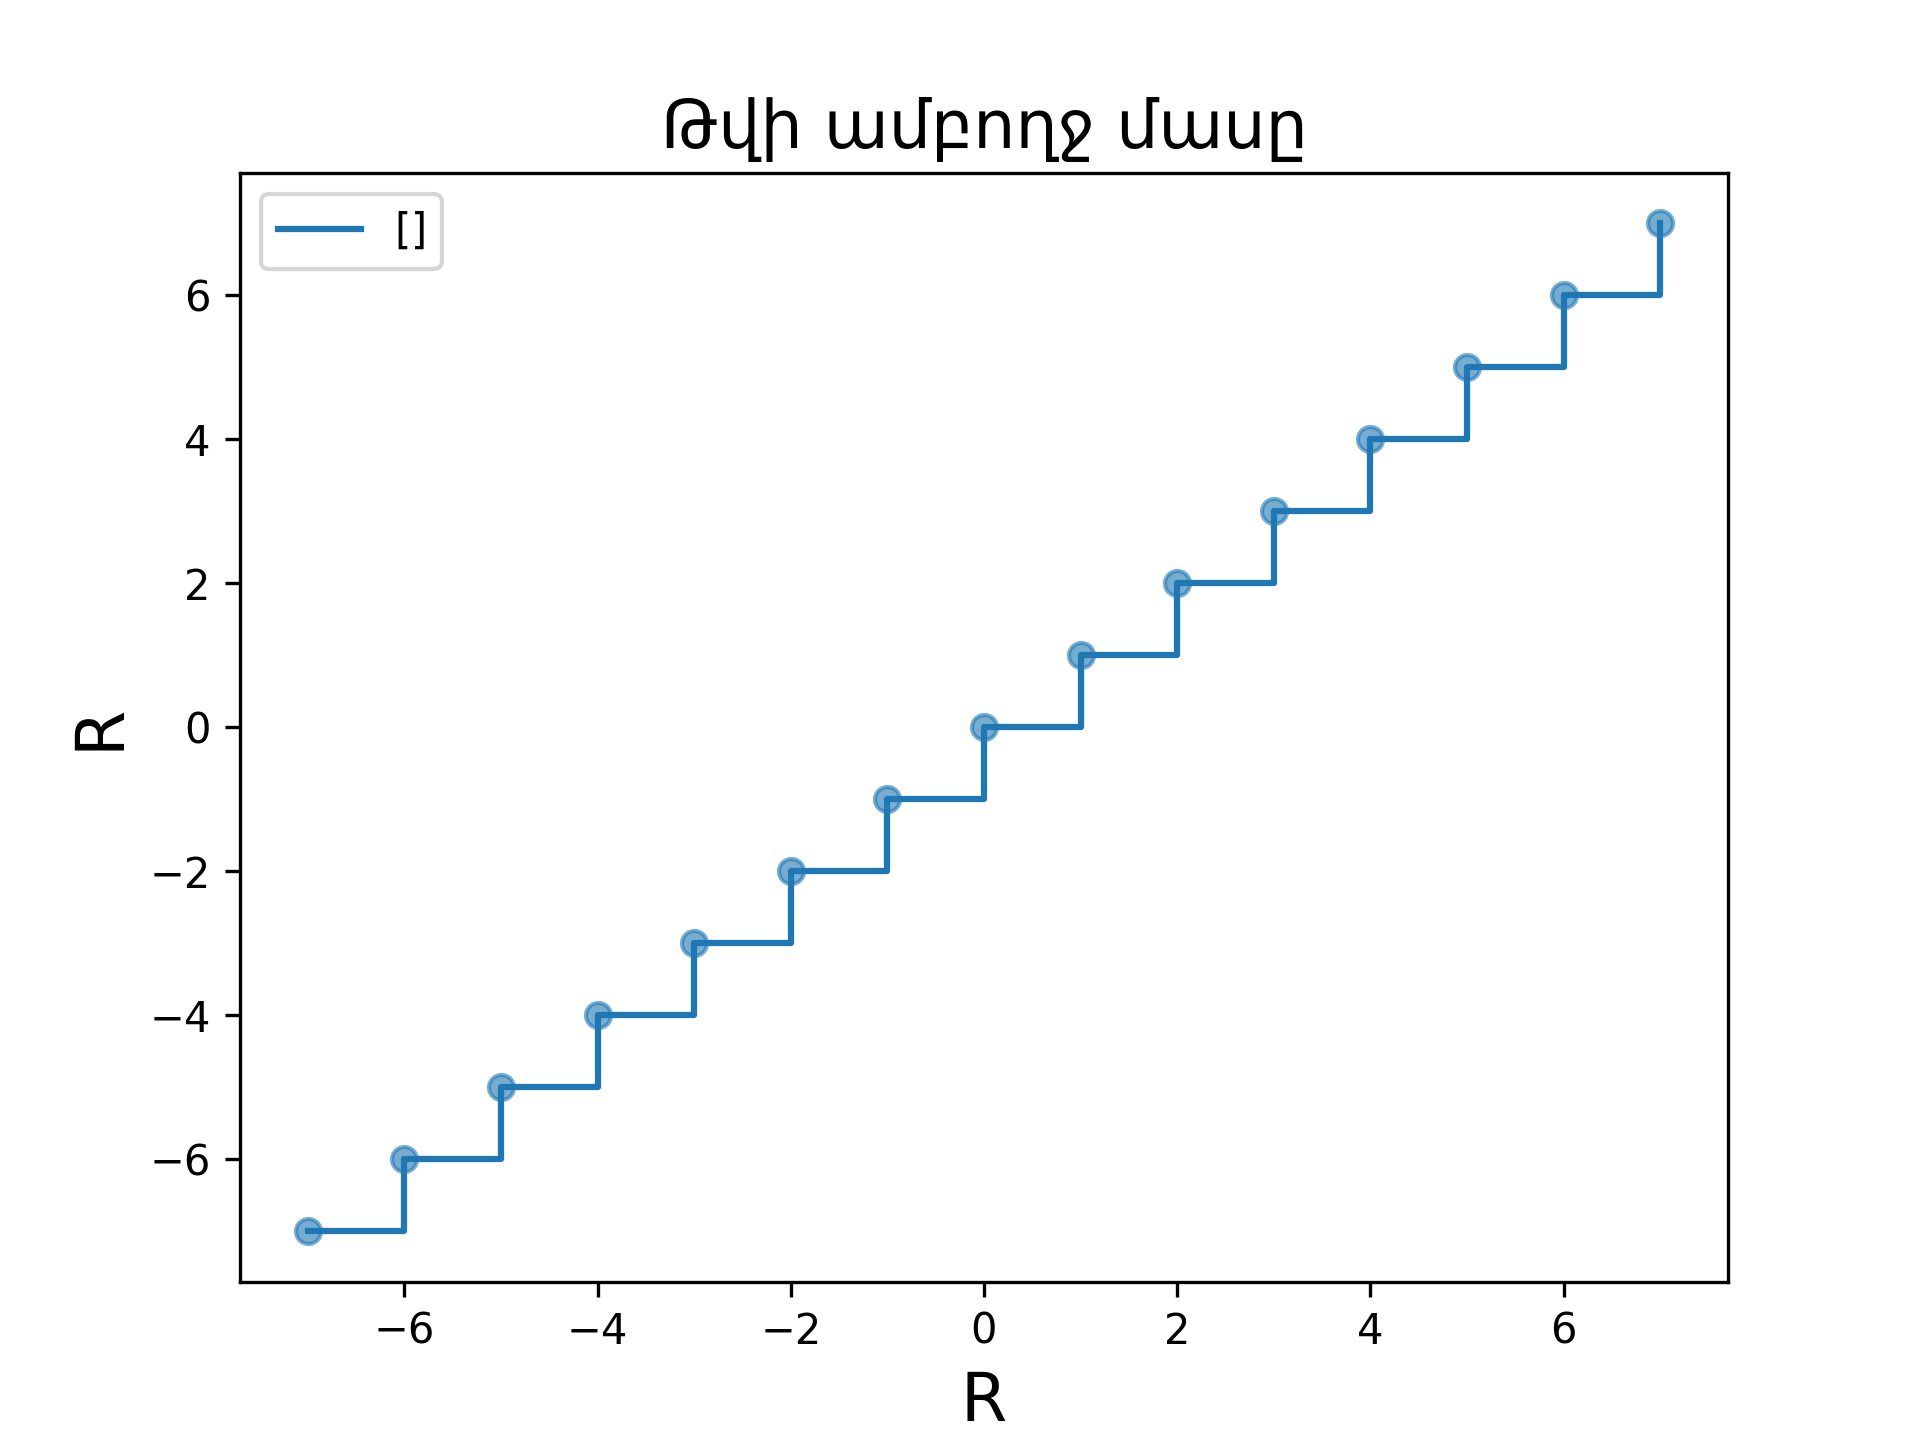
\includegraphics[width = 0.8\textwidth]{steps_None.png}}
                    \only<9>{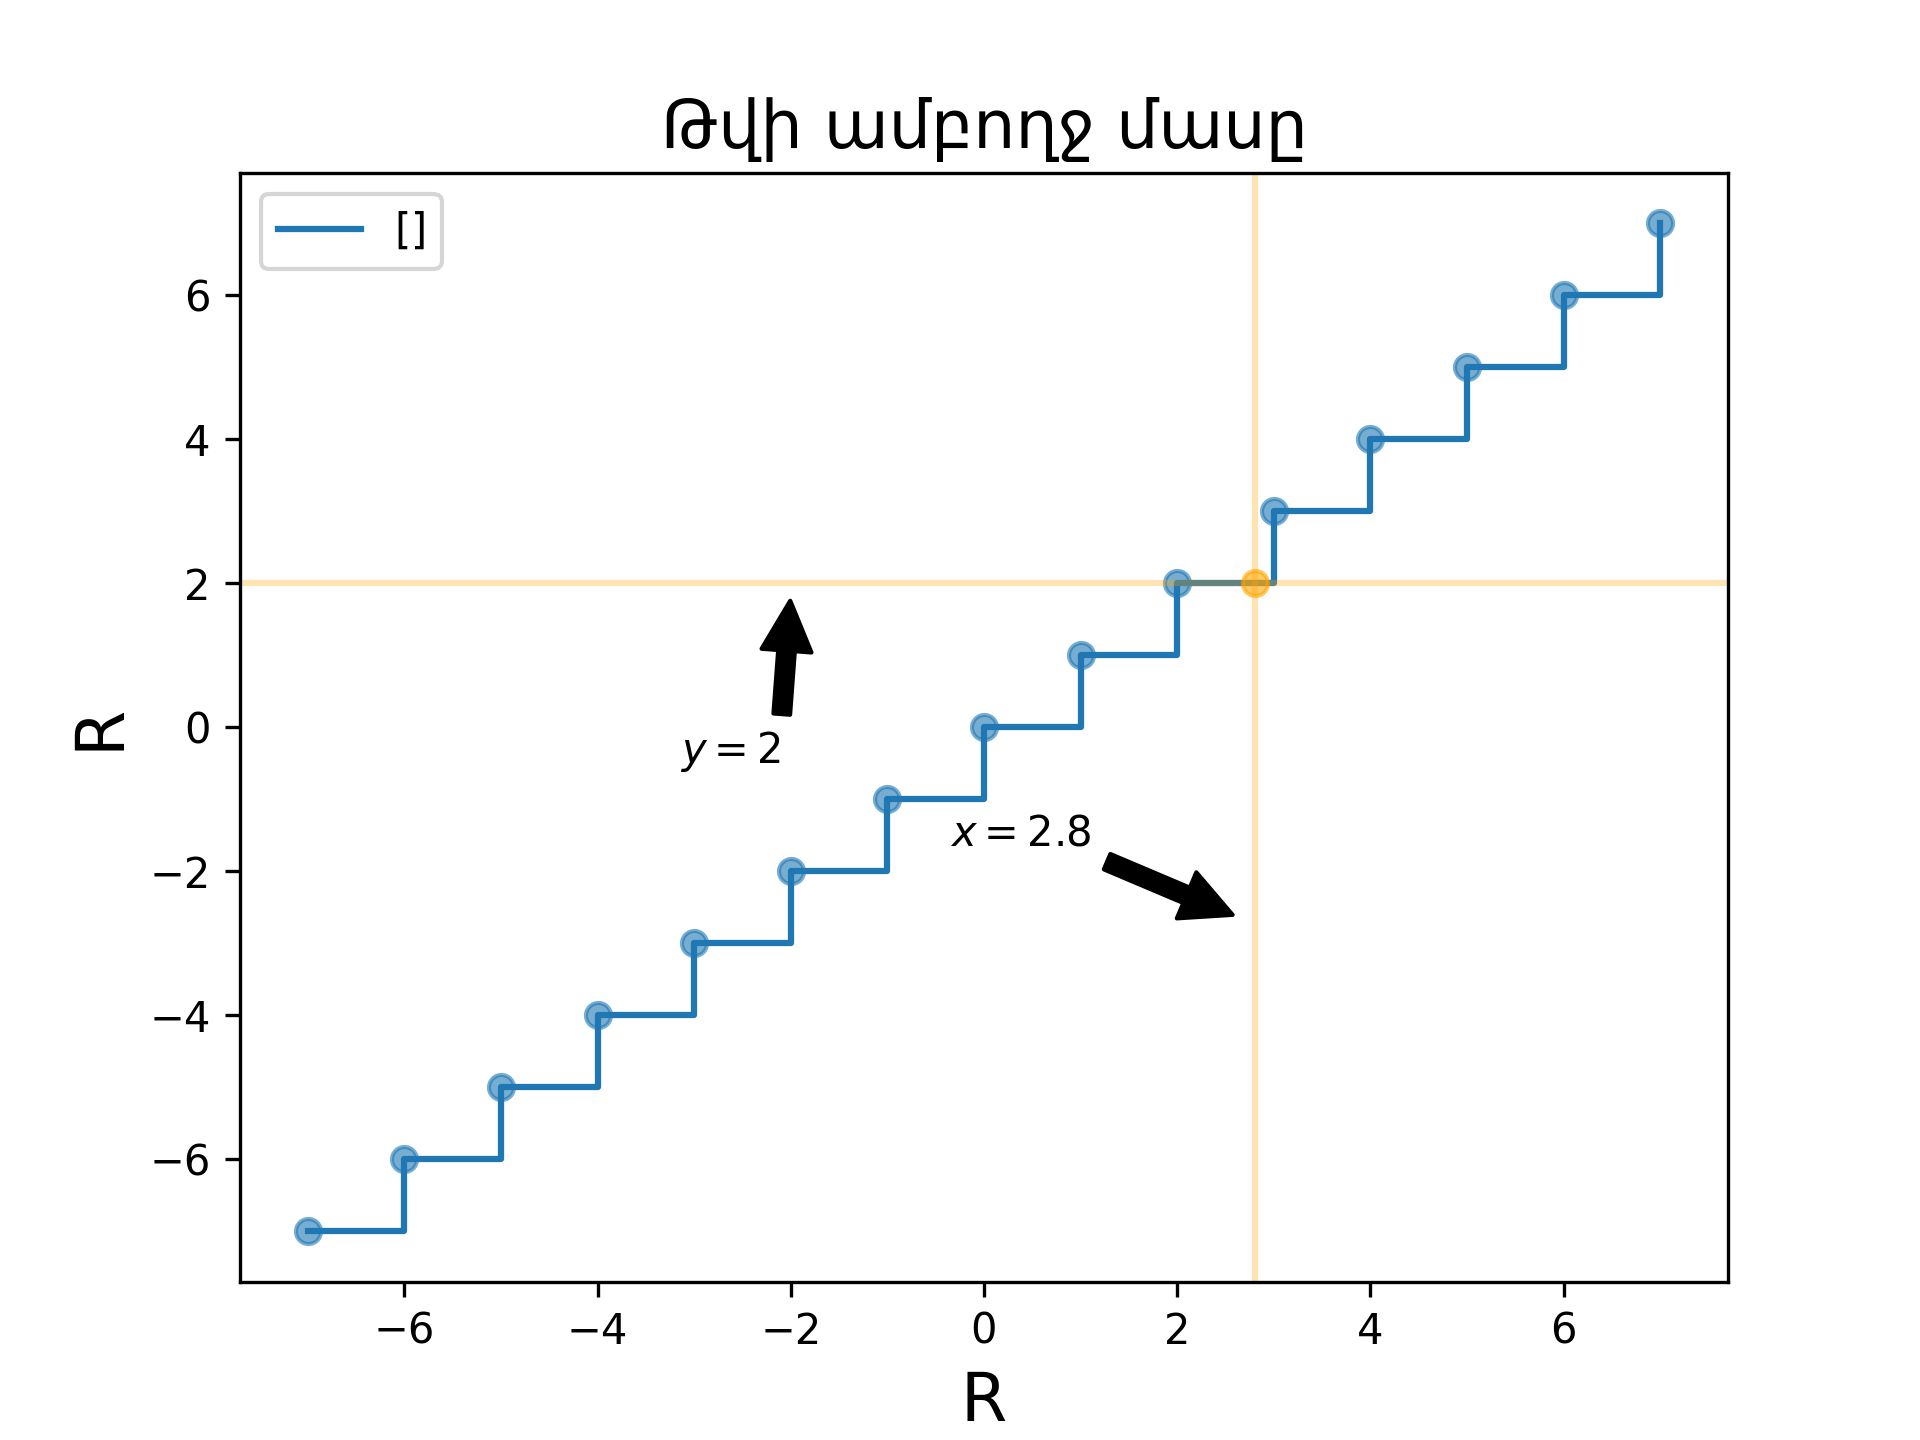
\includegraphics[width = 0.8\textwidth]{steps_2.8.png}}
                    \only<10>{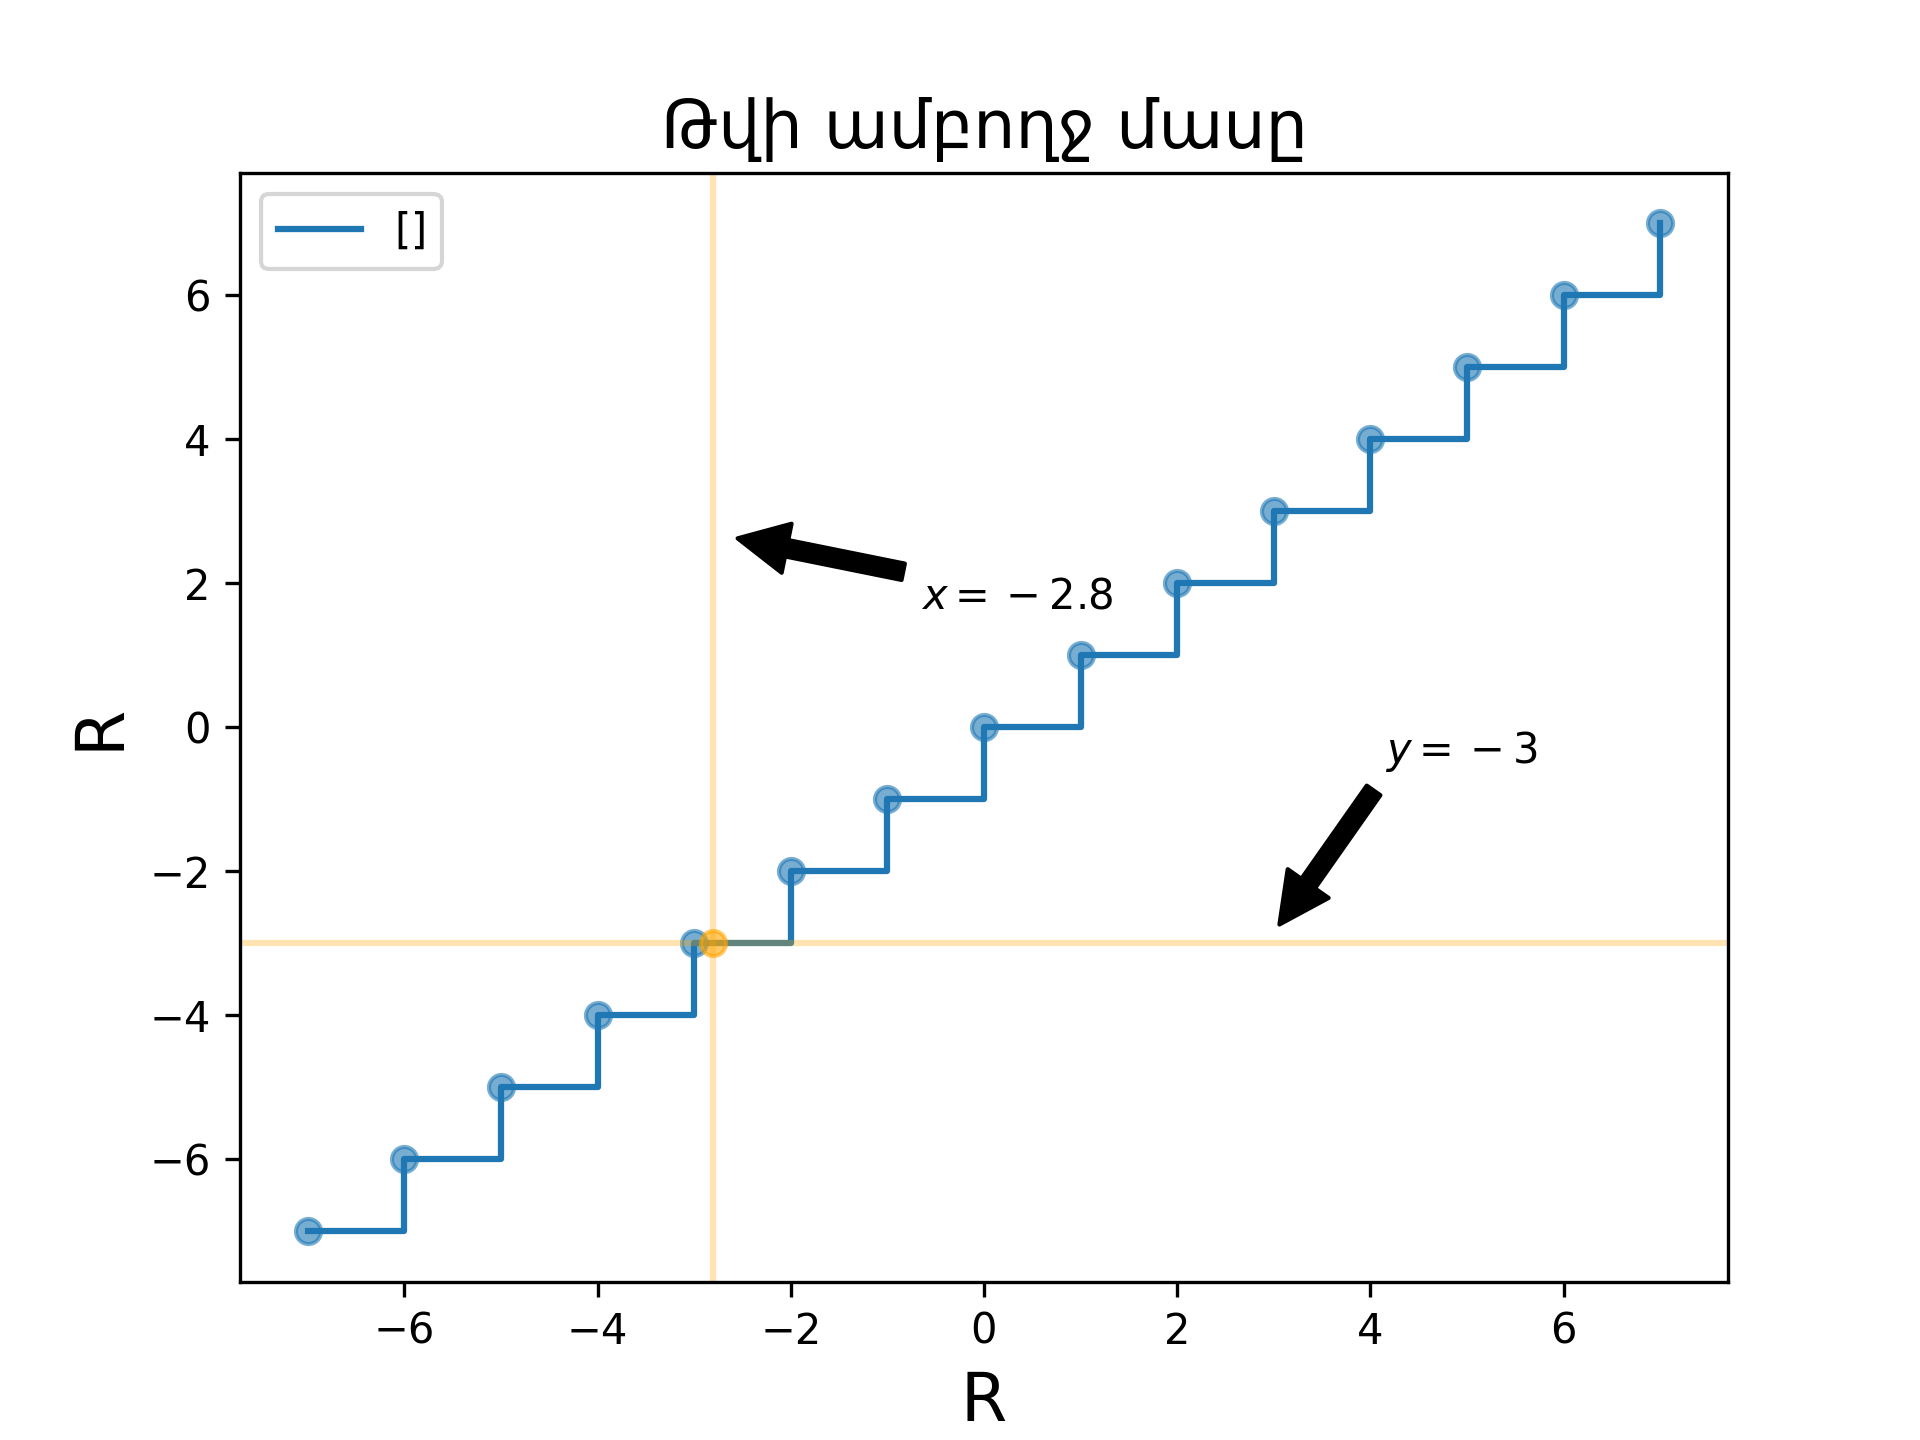
\includegraphics[width = 0.8\textwidth]{steps_-2.8.png}}
                \end{columns}
            }
        }
        \only<16>{
            \begin{exampleblock}{}
                Դիցուք $\alpha = \alert<6>{\pm}x_0.x_1x_2x_3...$: Ըստ Կանտորի կառուցման $\alpha$ թվի նախատիպ է հանդիսանում $(a_n)$ ֆունդամենտալ հաջորդականությունը, որտեղ․
                \[a_n = \alert<6>{\pm}x_0.x_1...x_n = \pm\frac{[|\alpha|10^n]}{10^n} = \sum_{i=0}^n\pm\frac{x_i}{10^i}:\]
            \end{exampleblock}
        }
        \only<11, 15>{
            \begin{block}{Նշանակում}
                Մի քանի էլեմենտների գումարի կարճ գրելաձևը․
                \[b_1 + b_2 + ... + b_n = \sum_{i \in \{1, 2, ..., n\}}b_i = \sum_{i=1}^nb_i\]
            \end{block}
        }
        \only<12>{
            \begin{exampleblock}{}
                $1$-ից $10$ թվերի գումարը $(b_i = i)$․
                \[\sum_{i=1}^{10}i = 1+2+...+10=55\]
            \end{exampleblock}
        }
        \only<13>{
            \begin{exampleblock}{}
                $1$-ից $10$ թվերի քառակուսիների գումարը $(b_i = i^2)$․
                \[\sum_{i=1}^{10}i^2 = 1^2+2^2+...+10^2=385\]
            \end{exampleblock}
        }
        \only<14>{
            \begin{exampleblock}{}
                $1$-ից $10$ թվերի հակադարձների գումարը $(b_i = \frac{1}{i})$․
                \[\sum_{i=1}^{10}\frac{1}{i} = \frac{1}{1}+\frac{1}{2}+...+\frac{1}{10}=\frac{7381}{2520}\approx2.93\]
            \end{exampleblock}
        }
        \only<16>{
            \begin{alertblock}{}
                Որոշ թվեր կարելի է գրել երկու տարբեր ձևերով:
                Չկա այնպիսի $\alpha$ իրական թիվ, որ
                \[
                    0.999(9) < \alpha < 1
                \]
            \end{alertblock}
        }
    \end{frame}
    \begin{frame}
        \frametitle{Իրական թվեր}
        \framesubtitle{Սահմանումը ըստ Դեդեկինդի}
        \only<1>{\centering 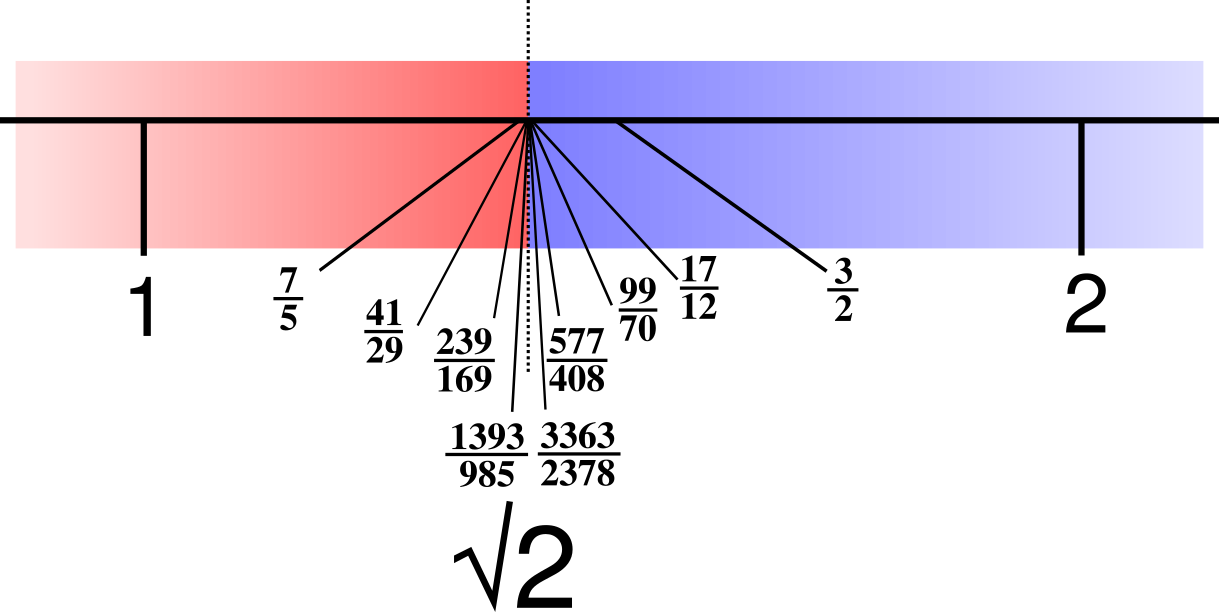
\includegraphics[width=0.5\textwidth]{dedekind_cut.png}}
        \only<2->{Իրական թվի նախատիպ է հանդիսանում ռացիոնալ թվեր տրոհումը երկու դասի այնպես, որ} 
        \begin{columns}
            \column{0.4\textwidth}
            \begin{itemize}
                \item<2-7>{\alert<5>{դասերը դատարկ չեն}}
                \only<2-7>{
                \item<3-7>{\alert<6>{յուրաքանչյուր ռացիոնալ թիվ միայն դասերից մեկում է}}
                \item<4-7>{\alert<7>{դասերից մեկի բոլոր թվերը մեծ են մյուս դասի բոլոր թվերից}}}
            \end{itemize}
            \only<8->{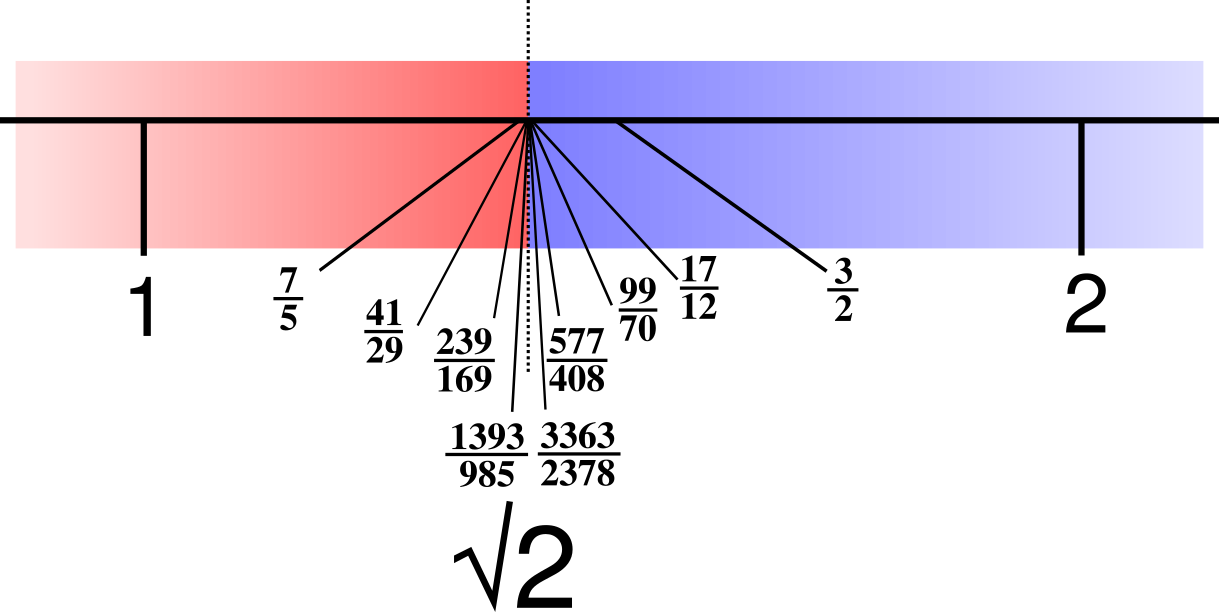
\includegraphics[width=0.95\textwidth]{dedekind_cut.png}}
            \column{0.4\textwidth}
            \only<5->{
            \begin{itemize}
                \item<5->{\alert<5>{$A, A' \neq \emptyset$}}
                \item<6->{\alert<6>{$A \cap A' = \emptyset$, և $A \cup A' = \mathbb{Q}$}}
                \item<7->{\alert<7>{$\forall a \in A \; \forall a' \in A': \; a < a'$}}
            \end{itemize}}
        \end{columns}
    \end{frame}
    \begin{frame}
        \frametitle{Իրական թվեր}
        \framesubtitle{Աքսիոմատիկ սահմանումը}
        \only<1>{
        \begin{exampleblock}{Աքսիոմները}
            Կարևոր չէ առարկաների էությունը, կարևոր է միայն գոյություն ունեցող հարաբերությունները նրանց միչև։
            \begin{itemize}
                \item{հանրահաշվական կառուցվածքի աքսիոմներ}
                \item{կարգավորվածության աքսիոմներ}
                \item{անընդհատության աքսիոմներ}
            \end{itemize}
        \end{exampleblock}
        }
        \only<2-14>{
        \begin{exampleblock}{Հանրահաշվական կառուցվածքի աքսիոմներ}
        \begin{columns}
            \column{0.5\textwidth}
            Գումար՝ $+: \mathbb{R} \times \mathbb{R} \rightarrow \mathbb{R}$
            \only<3->{
            \begin{itemize}
                \item<3->{Տեղափոխականություն}
                \only<4->{$\forall a, b \in \mathbb{R} \; a+b = b+a$}
                \item<5->{Զուգորդականություն}
                \only<6->{$\forall a, b, c \in \mathbb{R} \; (a+b)+c = a+(b+c)$}
                \item<7->{Կա $0$ թիվը\\}
                \only<8->{$\exists 0 \in \mathbb{R} \; \forall a \in \mathbb{R} \; 0+a = a$}
                \only<9->{\item<9->{Բոլոր թվերը ունեն իրենց հակդիր թիվը\\}
                \only<10->{$\forall a \in \mathbb{R} \; \exists -a\in \mathbb{R} \; -a+a = 0$}}
            \end{itemize}}
            \column{0.5\textwidth}
            Արտադրյալ՝ $\cdot : \mathbb{R} \times \mathbb{R} \rightarrow \mathbb{R}$
            \only<3->{
            \begin{itemize}
                \item<3->{Տեղափոխականություն}
                \only<4->{$\forall a, b \in \mathbb{R} \; a\cdot b = b\cdot a$}
                \item<5->{Զուգորդականություն}
                \only<6->{$\forall a, b, c \in \mathbb{R} \; (a\cdot b)\cdot c = a\cdot (b\cdot c)$}
                \item<7->{Կա $1$ թիվը\\}
                \only<8->{$\exists 1 \in \mathbb{R} \; \forall a \in \mathbb{R} \; 1\cdot a = a$}
                \only<9->{\item<9->{Բոլոր թվերը \alert<11>{բացի $0$-ից} ունեն հակադարձ}
                \only<10->{$\forall a \in \mathbb{R} \setminus \{0\}\; \exists a^{-1}\in \mathbb{R} \; a^{-1}a = 1$}}
            \end{itemize}}
        \end{columns}
        \only<12->{
            \begin{center}
            \begin{minipage}{0.4\textwidth}
                \begin{itemize}
                    \item<12->{Բաշխականություն\\}
                    \only<13->{$\forall a, b, c \in \mathbb{R} \; a\cdot (b+c) = a\cdot b + a\cdot c$}
                    \item<14->{$1 \neq 0$}
                \end{itemize}
            \end{minipage}
            \end{center}
        }
        \end{exampleblock}
        }
        \only<15-25>{
        \begin{exampleblock}{Կարգավորվածության աքսիոմներ}
        Թվերը կարելի է համեմատել․
        \only<16->{\begin{itemize}
            \item<16->{կամայական թիվ ինքն իրանից փոքր կամ հավասար է\\}
            \only<17->{$\forall a \in \mathbb{R}\; a \leq a$}
            \item<18->{կամայական երկու թիվ միաժամանակ փոքր հավասար են իրարից միայն այն դեպքում երբ իրար հավասար են\\}
            \only<19->{$\forall a, b \in \mathbb{R}$ եթե $a \leq b$ և $b \leq a$ ապա $a=b$}
            \item<20->{եթե $a$ թիվը փոքր է $b$ թվից, իսկ $b$ թիվը փոքր է $c$ թվից, ապա $a$ թիվը փոքր է $c$ թվից\\}
            \only<21->{$\forall a, b, c \in \mathbb{R}$ եթե $a \leq b$ և $b \leq c$ ապա $a\leq c$}
            \item<22->{գումարումը ու կարգավորվածությանը\\}
            \only<23->{$\forall a, b, c \in \mathbb{R}$ եթե $a \leq b$ ապա $a + c \leq b + c$}
            \item<24->{արտադրյալը ու կարգավորվածությանը\\}
            \only<25->{$\forall a, b, c \in \mathbb{R}$ եթե $a \leq b$ և $c \geq 0$ ապա $a \cdot c \leq b \cdot c$}
        \end{itemize}}
        \end{exampleblock}
        }
        \only<26-28>{
        \begin{exampleblock}{Անընդհատության աքսիոմը}
            \begin{itemize}
                \item{Կամայական $A \subset \mathbb{R}$ և $B \subset \mathbb{R}$ բազմությունները, որ բոլոր երկու $a\in A$ և $b\in B$ տարերի համար տեղի ունենա $a \leq b$ անհավասարությունը, միշտ \alert<28>{կգտնվի այնպիսի $\xi \in \mathbb{R}$}, որ կլինի մեծ կամ հավասար $A$ բազմության բոլոր տարերից և փոքր կամ հավասար՝ $B$ բազմության տարերից\\}
            \end{itemize}
                \only<26>{\centering 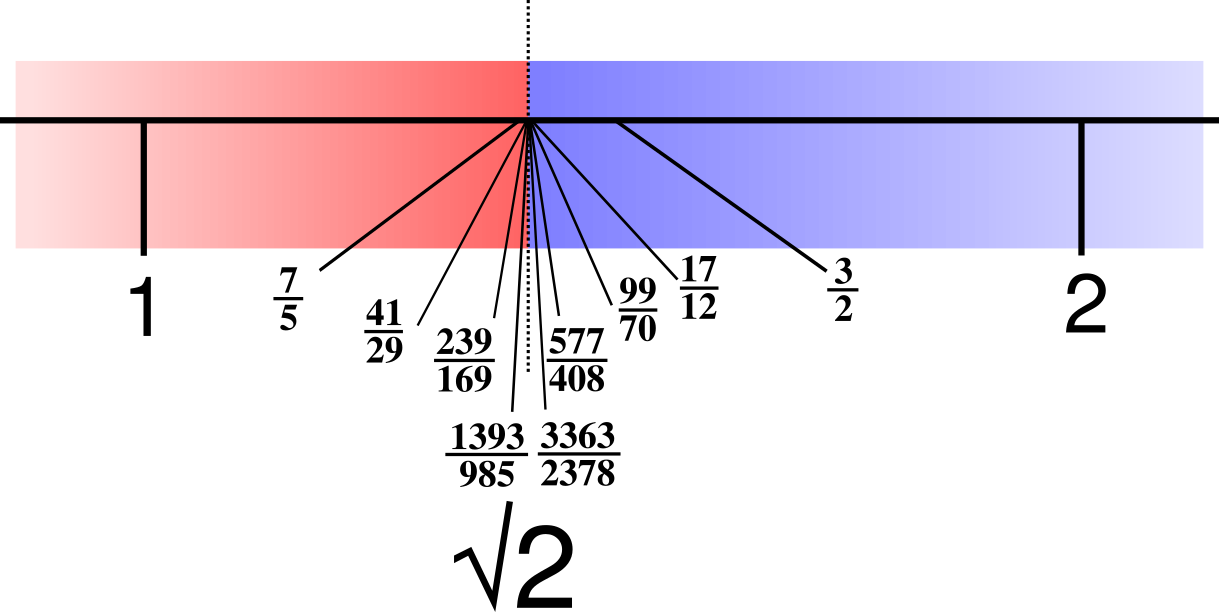
\includegraphics[width=0.3\textwidth]{dedekind_cut.png}}
        \end{exampleblock}
        }
        \only<27->{
            \begin{exampleblock}{Օրինակ}
                Դիցուք՝ \alert<41>{$A = \{q \in \mathbb{Q}: \alert<31>{q^2 < 2 \text{ կամ } q < 0}\}$} և $B = \{q \in \mathbb{Q}: q^2 \geq 2 \text{ և } \alert<30>{q \geq 0}\}$:\\
                Չնայած նրա, որ \alert<29>{$\forall a \in A$ և $\forall b \in B$ ճիշտ է $a \leq b$}, \alert<38>{գոյություն չունի այնպիսի \alert<28>{$\xi \in \mathbb{Q}$}}, որ $\forall a \in A$ և $\forall b \in B$ տեղի ունենա
                \only<27-28>{\[a \leq \xi \leq b\]} \only<29->{$a \leq \xi \leq b$}
                անհավասարությունը։
            \end{exampleblock}
        }
        \only<29->{
            \begin{alertblock}{Ապացույց}
                \only<29-37>{Համոզվենք, որ $\forall a \in A$ և $\forall b \in B$ ճիշտ է $a \leq b$ անհավասարությունը։\\
                \only<30->{\begin{itemize}
                    \item{Եթե $a \leq 0$, ապա $a \leq 0 \leq b$:}
                    \only<31->{\item{Եթե $a > 0$, ապա $a^2 < 2$ } \only<32->{Հաշվի առնելով, որ $a > 0$ և $b \geq 0$, ունենք, որ}}
                    \only<33-36>{\[b - a = \frac{\alert<35>{(b-a)}\alert<34-35>{(b+a)}}{\alert<34>{b+a}} = \frac{\alert<36>{b^2-a^2}}{b+a} >  \frac{0}{a+b} = 0:\]}
                    \only<37->{\[b - a = \frac{(b-a)(b+a)}{b+a} = \frac{b^2-a^2}{b+a} \alert{\underbrace{>}_{b^2 \geq 2 > a^2 \text{ և } a + b > 0}}  \frac{0}{a+b} = 0:\]}
                \end{itemize}}}
                \only<38->{
                    Դիցուք՝ կա այնպիսի $\xi \in \mathbb{Q}$, որ \alert<42>{$\forall a \in A$} և $\forall b \in B$ տեղի ունի $\alert<42>{a \leq \xi} \leq b$։\\
                    % \only<37->{Եթե $\xi^2 \neq 2$, ապա կամ՝ $\xi^2 < 2$, կամ՝ $\xi^2 > 2$։\\}
                    \only<39, 55->{$\xi^2$ կարող է լինել՝
                    \begin{itemize}
                        \item {$\xi^2 < 2$ \only<55->{ հակասություն $\xi < \xi + \delta \in A$}}
                        \item {$\xi^2 > 2$ \only<56->{ հակասություն $\xi > \xi - \delta \in B$}}
                        \item {\alert<57>{$\xi^2 = 2$} \only<58->{ հակասություն $\xi \notin \mathbb{Q}$}}
                    \end{itemize}}
                    \only<40-54>{Եթե \alert<40>{$\xi^2 < 2$}, \alert<43>{կա} $\alert<43>{\delta} \in {\mathbb{Q}_{+}}=\{q \in \mathbb{Q}: q > 0\}$ այնպիսի որ \alert<41>{$(\xi + \delta)^2 < 2$}\only<-42>{, կունենաք հակասություն}\only<41-42>{, $(\xi + \delta) \in A$}\only<42>{, բայց $(\xi + \delta) \nleq \xi$}։\\}
                    \only<44>{\[(\xi + \delta)^2 = \xi^2 + 2 \xi \delta + \delta^2\]}
                    \only<45>{\[(\xi + \delta)^2 = \xi^2 + \alert{\underbrace{2 \xi \delta + \delta^2}_{\text{եթե փոքր է } 2 - \xi^2 > 0}}\]}
                    \only<46>{\[(\xi + \delta)^2 = \xi^2 + \underbrace{2 \xi \delta + \delta^2}_{\text{եթե փոքր է } 2 - \xi^2 > 0} < \xi^2 + 2 - \xi^2\]}
                    \only<47-48>{\[(\xi + \delta)^2 = \xi^2 + \underbrace{2 \xi \delta + \delta^2}_{\text{եթե փոքր է } 2 - \xi^2 > 0} < 2\]}
                    \only<48-53>{Գտնենք $\delta$ բավարարող \alert<40>{$2 \xi \delta + \delta^2 < 2 - \xi^2$} անհավասարությունը:\\}
                    \only<49-53>{Երբ $0 < \delta < 1$ ունենք որ $\delta^2 < \delta$}
                    \only<50>{
                        \[2 \xi \delta + \delta^2 < 2 \xi \delta + \delta\]
                    }
                    \only<51>{
                        \[2 \xi \delta + \delta^2 < (2\xi + 1)\delta\]
                    }
                    \only<52>{
                        \[2 \xi \delta + \delta^2 < \alert{(2\xi + 1)\delta < 2 - \xi^2}\]
                    }
                    \only<53>{
                        \[2 \xi \delta + \delta^2 < (2\xi + 1)\delta \alert{\underbrace{<}_{\text{երբ } \delta < \frac{2-\xi^2}{2\xi + 1}}} 2 - \xi^2\]
                    }
                    \only<54>{Երբ $0<\delta < \min\left\{\frac{2-\xi^2}{2\xi + 1}, 1\right\}$, կունենանք որ $(\xi + \delta)^2 < 2$}
                }
            \end{alertblock}
        }
    \end{frame}

    \begin{frame}
        \frametitle{Արամատ երկու}
        \framesubtitle{Իռացիոնալ թվեր}
        \begin{block}{Պնդում}
            Թիվ, որի քառակուսին $2$ է ռացիոնալ չէ։\\
            \[\xi^2 = 2 \; \xi \notin \mathbb{Q}\]
        \end{block}
        \only<2->{
            \begin{alertblock}{Ապացույց}
                \only<2-5>{
                    Դիցուք՝ $\xi^2 = 2$ և $\xi \in \mathbb{Q}$։\\
                }
                \only<3-5>{Եթե $\xi \in \mathbb{Q}$, ապա \[\xi = \frac{n}{m}\] որտեղ $n$ և $m$ թվերի ընդհանուր ամենամծ բաժանարարը $1$ է։\\}
                \only<4-5>{\[\only<5->{\alert<5>{m^2}}\xi^2 = \frac{\only<5->{\alert<5>{m^2}}n^2}{m^2} = \only<5->{\alert<5>{m^2}}2\]}
                \only<6->{\[\alert<12>{n^2 = \alert<7>{2} m^2}\] որտեղ \alert<16>{$n$ և $m$ թվերի ընդհանուր ամենամծ բաժանարարը $1$ է}։\\}
                \only<13->{Քանի որ }\only<7->{$n^2$ զույգ թիվ է}\only<8->{, $n$-ը ևս զույգ թիվ է}\only<9-11>{ քանի որ կենտ թվի քառակուսին կենտ է․}
                \only<10>{\[(\underbrace{2k+1}_{\text{կենտ թիվ}})^2 = 4k^2 + 4k + 1\]}
                \only<11>{\[(2k+1)^2 =  \underbrace{\alert{2}(2k^2 + 2k) + 1}_{\text{կենտ թիվ}}\]}
                \only<12>{\[n = 2k\]}
                \only<13>{\[(2k)^2 = 2 m^2\]}
                \only<14>{\[4k^2 = 2 m^2\]}
                \only<15->{\[2k^2 = m^2\]}
                \only<15->{Քանի որ $m^2$ զույգ թիվ է, $m$-ը ևս զույգ թիվ է}

            \end{alertblock}
        }
    \end{frame}

    \begin{frame}
        \frametitle{Անընդհատության աքսիոմի հետևանքները}
        \framesubtitle{Ճշգրիտ վերին եզր}
        \only<1->{
            \begin{block}{Պնդում}
                Կամայական \alert<2>{վերևից սահմանափակ} իրական թվերի ենթաբզմություն ունի \alert<6>{ճշգրիտ \alert<5>{վերին եզր}}։
            \end{block}
        }
        \only<3-5>{
            \begin{block}{Սահմանում}
                Բազմությունը \alert<3>{վերևից սահմանափակ} է, եթե գոյություն ունի այնպիսի թիվ, որ բազմության բոլոր թվերից մեծ կամ հավասար է։
            \only<4->{\[A \subset \mathbb{R} \text{ վերևից սահմանափակ է, եթե } \exists M \in \mathbb{R}: \; \forall a \in A \; a \leq M\]}
            \only<5->{$M$ թիվը կոչվում է \alert<5>{վերի եզր}}
            \end{block}
        }
        \only<6-13>{
            \begin{block}{Սահմանում}
                Բազմության \alert<6>{ճշգրիտ վերին եզր} է կոչվում, վերին եզրերից փոքրագույնը։\\
                \only<7->{
                    Եթե $S$-ը $A$ բազմության ճշգրիտ վերին եզրն է, ապա՝
                    \only<8->{\begin{itemize}
                        \only<8->{\item{$S$-ը վերին եզր է $A$ բազմության համար\\}}
                        \only<9->{$\forall a \in A \; a \leq S$}
                        \only<10->{\item{\alert<13>{$S$-ից փոքր կամայական թիվ} $A$ բազմության համար վերին եզր չէ\\}}
                        \only<11>{$\forall s < S\;  \exists a_s  \in A\; a_s > s$}
                        \only<12>{$\forall s < S\;  \exists a_s  \in A\; a_s > s = S - \varepsilon$}
                        \only<13->{$\alert<13>{\forall \varepsilon > 0}\;  \exists a_s  \in A\; a > \alert<13>{S - \varepsilon}$}
                    \end{itemize}}
                }
            \end{block}
        }
        \only<14->{
            \begin{alertblock}{Ապացույց}
                \only<15-27>{Եթե $A$, և $B$ բազմությունները այնպիսին են, որ }
                \only<16-18>{\[\forall a \in A, \; \forall b \in B: \; a \leq b\]}
                \only<19-27>{\alert<26>{$\forall a \in A, \; \forall b \in B: \; a \leq b$}, }
                \only<17-27>{ապա}
                \only<18-21, 26-27>{\alert<27>{\[\exists \xi \in \mathbb{R}:\; \forall a \in A, \; \forall b \in B: \; a \leq \xi \leq b\]}}
                \only<22-25>{$\exists \xi \in \mathbb{R}:\; \forall a \in A, \; \forall b \in B: \; a \leq \xi \leq b$\\}
                \only<20->{Դիցուք $A$-ն վերևից սահմանափակ բազմություն է։\\}
                \only<21->{$B$-ով նշանակենք $A$-ին վերևից սահմանափակող թվերի բազմությունը։\\}
                \only<26-27>{$b \in B$ նշանակում է $b$-ն վերևից սահմանափակում է $A$ բազմությանը։\\}
                \only<28->{Համաձայն անընդհատության աքսիոմի․ \[\exists \xi \in \mathbb{R}:\; \alert<29>{\forall a \in A}, \; \alert<30>{\forall b \in B}: \; \alert<29>{a \leq} \alert<29-30>{\xi} \alert<30>{\leq b}\]}
                \only<29-30>{$\xi$-ն վերևից սահմանափակում է $A$ բազմությանը, $\xi \in B$։\\}
                \only<30>{$\xi$-ն վերին եզրերից փոքրագույնն է։\\}
                \only<31>{$\xi$-ն $A$ բազմության ճշգրիտ վերին եզրն է։\\}
            \end{alertblock}
            \only<22-25>{
                \begin{exampleblock}{Օրինակ}
                    $A = \{x\in \mathbb{R}:\; -1 < x < \pi\} =: (-1, \pi)$\\
                    \only<23>{$B = \{x \in \mathbb{R}:\; x \text{-ը վերևից սահմանափակում է } A \text{ բազմությունը}\}$}
                    \only<24>{$B = \{x \in \mathbb{R}: \; x\geq\pi\}$}
                    \only<25>{$B = \{x \in \mathbb{R}: \; x\geq\pi\} =: [\pi, +\infty) $}
                \end{exampleblock}
            }
        }
    \end{frame}

    \begin{frame}
        \frametitle{Անընդհատության աքսիոմի հետևանքները}
        \framesubtitle{Ներդրված հատվածնրի լեմմ}
        \only<1->{
            \begin{block}{Պնդում}
                Կամայական ներդրված \alert<8>{ոչ դատարկ} հատվածների հաջորդականություն համար, \only<-13>{\[\forall n \in \mathbb{N}: \; [a_{n+1}, b_{n+1}]\subset[a_n, b_n]\]} գոյություն ունի այնպիսի $c \in \mathbb{R}$ թիվ, որ պատկնում է բոլոր հատվածներին, այսինքն՝ \[\forall n \in \mathbb{N}\; c \in [a_n, b_n]:\]
            \end{block}
            \centering{
            \only<2>{\includegraphics[width=0.7\textwidth]{5b49576b/nested_intervals_1.png}}
            \only<3>{\includegraphics[width=0.7\textwidth]{5b49576b/nested_intervals_2.png}}
            \only<4>{\includegraphics[width=0.7\textwidth]{5b49576b/nested_intervals_3.png}}
            \only<5>{\includegraphics[width=0.7\textwidth]{5b49576b/nested_intervals_4.png}}
            \only<6>{\includegraphics[width=0.7\textwidth]{5b49576b/nested_intervals_5.png}}}
        }
        \only<7->{
            \begin{alertblock}{Ապացույց}
                \only<7-9>{Հիշենք, որ $[a_n, b_n] = \{x \in \mathbb{R}: \; a_n \leq x \leq b_n \}$:}
                \only<8>{\[a_n \leq b_n\]}
                \only<9>{\[\forall n \in \mathbb{N}: \; a_n \leq b_n\]}
                \only<10-13>{
                    Նկատենք, որ $[a_{n+1}, b_{n+1}]\subset[a_n, b_n]$ Նշանակում է
                    \only<11>{\[a_n \leq a_{n+1} \alert{\leq} b_{n+1} \leq b_{n}\]}
                    \only<12>{\[a_n \leq a_{n+1} \leq a_{n+2} \alert{\leq} b_{n+2} \leq b_{n+1} \leq b_{n}\]}
                    \only<13>{\[a_n \leq a_{n+1} \leq a_{n+2} \leq \cdots \leq a_{n+p} \alert{\leq} b_{n+p} \leq \cdots \leq b_{n+2} \leq b_{n+1} \leq b_{n}\]}
                }
                \only<14->{
                    \[a_1 \leq a_{2} \leq a_{3} \leq \cdots \leq a_{n} \leq \cdots \alert{\leq} \cdots \leq b_{n} \leq \cdots \leq b_{3} \leq b_{2} \leq b_{1}\]
                    \only<14->{$A := \{a_1, a_2, ...\}$-հատվածների ձախ ծայրակետերը։\\}
                    \only<15->{$B := \{b_1, b_2, ...\}$-հատվածների աջ ծայրակետերը։\\}
                    \only<16->{Քանի որ $\forall a \in A, b \in B: \; a \leq b$\only<17->{,} }
                    \only<17>{համաձայն անընդհատության աքսիոմի \[\exists \xi \in \mathbb{R}: \; \forall a \in A, b \in B \; a \leq \xi \leq b\]}
                    \only<18->{համաձայն անընդհատության աքսիոմի \[\exists \xi \in \mathbb{R}: \; \forall a \in A, b \in B \; \xi \in [a, b]\]}
                    \only<19->{\[\forall n \in \mathbb \; \xi \in [a_n, b_n]\]}
                }
            \end{alertblock}
        }
    \end{frame}

    \begin{frame}
        \frametitle{Իրական թվերը անհաշվելի են}
        \only<1-5, 13->{
            \begin{block}{Սահմանում}
                $A$ բազմությունը \alert<1, 4>{հաշվելի} է, \only<-2>{\alert<2>{եթե նրա տարրերը կարելի է համարակալե բնական թվերով:}}
                \only<3->{եթե $A$ և $\mathbb{N}$ բազմություննեի միջև գոյություն ունի \alert<4>{փոխմիարժեք արտապատկերում}։}
            \end{block}
        }
        \only<5-13>{
            \begin{block}{Սահմանում}
                $f:A \rightarrow B$ արտապատկերումը \alert<5>{փոխմիարժեք} է, եթե կամայական $b \in B$ տարրի \alert<6-9>{նախապատկերում} կա մեկ տարր\only<13>{։}
                \only<-13>{\[f^{-1}(\{b\}) := \{a\in A: \; f(a) \in \{b\}\}:\]}
                Այսինքն $f(x) = b$ ունի մեկ լուծում։
            \end{block}
        }
        \only<6-12>{
        \begin{columns}
            \column{0.5\textwidth}
            \only<6->{\[f: \mathbb{R} \rightarrow \mathbb{R}\]}
            \only<7-8>{\[f^{-1}([y_1, y_2])\]}
            \only<9>{\[f^{-1}([y_1, y_2]) = [x_1, x_2] \cup [x_3, x_4]\]}
            \only<10->{Իսկ $[x_1, x_2]$ բազմության \alert{պատկեր} անվանում են՝}
            \only<11>{\[f([x_1, x_2]) := \{f(x) \in \mathbb{R}: x \in [x_1, x_2]\}\]}
            \only<12>{\[f([x_1, x_2]) = [y_1, y_2]\]}
            \column{0.4\textwidth}
            \only<6>{\includegraphics[width=0.95\textwidth]{5b49576b/func_preimage_plot_0.png}}
            \only<7>{\includegraphics[width=0.95\textwidth]{5b49576b/func_preimage_plot_1.png}}
            \only<8>{\includegraphics[width=0.95\textwidth]{5b49576b/func_preimage_plot_2.png}}
            \only<9>{\includegraphics[width=0.95\textwidth]{5b49576b/func_preimage_plot_3.png}}
            \only<10>{\includegraphics[width=0.95\textwidth]{5b49576b/func_image_plot_1.png}}
            \only<11>{\includegraphics[width=0.95\textwidth]{5b49576b/func_image_plot_2.png}}
            \only<12>{\includegraphics[width=0.95\textwidth]{5b49576b/func_image_plot_3.png}}
        \end{columns}
        }
        \only<13->{
            \begin{block}{Պնդում}
                Իրական թվերի բազմությունը \alert<14>{անհաշվելի է}։ Կամայական $f: \mathbb{N} \rightarrow \mathbb{R}$ արտապատկերման համար կգտնվի այպիսի \alert<14>{$\xi \in \mathbb{R}$, որ $f(n) = \xi$ լուծում չունի}։
            \end{block}
        }
        \only<14>{\includegraphics[width=0.95\textwidth]{5b49576b/nested_intervals_special_1.png}}
        \only<15>{\includegraphics[width=0.95\textwidth]{5b49576b/nested_intervals_special_cut3_1.png}}
        \only<16>{\includegraphics[width=0.95\textwidth]{5b49576b/nested_intervals_special_check_1.png}}
        \only<17>{\includegraphics[width=0.95\textwidth]{5b49576b/nested_intervals_special_2.png}}
        \only<18>{\includegraphics[width=0.95\textwidth]{5b49576b/nested_intervals_special_cut3_2.png}}
        \only<19>{\includegraphics[width=0.95\textwidth]{5b49576b/nested_intervals_special_check_2.png}}
        \only<20>{\includegraphics[width=0.95\textwidth]{5b49576b/nested_intervals_special_3.png}}
        \only<21>{\includegraphics[width=0.95\textwidth]{5b49576b/nested_intervals_special_cut3_3.png}}
        \only<22>{\includegraphics[width=0.95\textwidth]{5b49576b/nested_intervals_special_check_3.png}}
        \only<23>{\includegraphics[width=0.95\textwidth]{5b49576b/nested_intervals_special_4.png}}
        \only<24>{\includegraphics[width=0.95\textwidth]{5b49576b/nested_intervals_special_cut3_4.png}}
        \only<25>{\includegraphics[width=0.95\textwidth]{5b49576b/nested_intervals_special_check_4.png}}
        \only<26>{\includegraphics[width=0.95\textwidth]{5b49576b/nested_intervals_special_5.png}}
        \only<27>{\includegraphics[width=0.95\textwidth]{5b49576b/nested_intervals_special_cut3_5.png}}
        \only<28>{\includegraphics[width=0.95\textwidth]{5b49576b/nested_intervals_special_check_5.png}}
    \end{frame}

\end{document}